\documentclass{standalone}
\usepackage{tikz}
\usetikzlibrary{shapes,arrows,positioning,shapes.misc,shapes.geometric}
\usetikzlibrary{matrix}
\begin{document}
	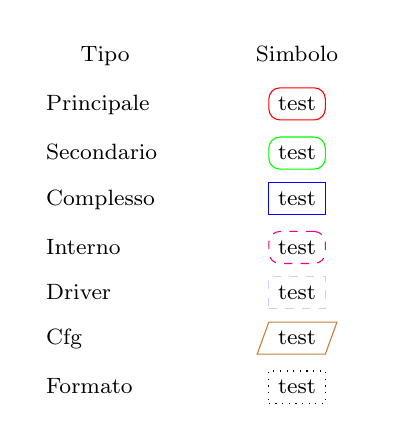
\begin{tikzpicture}
\tikzset{base/.style={text=black, align=center,text=black,draw,minimum size=1mm}, }	
\tikzset{testobase/.style={font=\footnotesize,minimum  width=1.0em, align=left}, }
\tikzset{testo/.style={testobase,text width=15mm}, }
\tikzset{main node/.style={testobase,base, draw=red, rounded corners}, }
\tikzset{main2 node/.style={testobase,base, draw=green,rounded corners}, }
\tikzset{complesso node/.style={testobase,base, draw=blue}, }
\tikzset{internal node/.style={testobase,base, draw=magenta,dashed,rounded corners}, }
\tikzset{driver node/.style={testobase,base,dashed,draw=blue!20}, }
\tikzset{formato node/.style={testobase,base,dotted}, }
\tikzset{cfg node/.style={testobase,base,trapezium,,trapezium left angle=70,trapezium right angle=-70,draw=brown}, }
\tikzset{linea/.style={-triangle 90},}

% \tikzset{base/.style={align=center,text=black}, }	
% %\tikzset{testobase/.style={minimum  width=1.0em, }, }
% \tikzset{testo/.style={,align=left}, }
% \tikzset{main node/.style={,base, draw=red, rounded corners}, }
% \tikzset{main2 node/.style={,base, draw=green,rounded corners}, }
% \tikzset{complesso node/.style={,base, draw=blue}, }
% \tikzset{internal node/.style={,base, draw=magenta,dashed,rounded corners}, }
% \tikzset{driver node/.style={,base,dashed,draw=blue!20}, }
% \tikzset{formato node/.style={,base,dotted}, }
% \tikzset{cfg node/.style={,base,trapezium,,trapezium left angle=70,trapezium right angle=-70,draw=brown}, }
% \tikzset{linea/.style={-triangle 90},}
	\matrix(tabella)[matrix of nodes,column sep=1em, row sep=.4em]
	{
\node[testo,align=center] (a){Tipo};&&\node[testo,align=center] (b){Simbolo};\\
\node[testo] (1){Principale}; &&\node[main node] (2){test}; \\
\node[testo] (3) {Secondario};&&\node[main2 node] (4){test};\\
\node[testo] (5) {Complesso}; &&\node[complesso node] (6){test};\\
\node[testo] (7) {Interno}; &&\node[internal node] (8){test};\\
\node[testo] (9) {Driver};&&\node[driver node] (10){test};\\
\node[testo] (11) {Cfg};&&\node[cfg node] (12){test};\\
\node[testo] (13) {Formato};&&\node[formato node] (14){test};\\
	};
	\end{tikzpicture}
\end{document}